
\documentclass[
  ngerman
  ,12pt
  ,pdftex
]{article}

\usepackage{graphicx}
\usepackage{amsmath}
\usepackage{amssymb}
\usepackage{listings}
\usepackage{a4wide}
\usepackage{float}
\usepackage{color}
\usepackage{tikz}
\usepackage[ngerman]{babel}
\usepackage[utf8]{inputenc}
\usepackage[T1]{fontenc}
\usepackage{comment}
\usepackage{lstlangarm}

\usepackage{pdfpages}






\lstdefinestyle{myStyle}{
    belowcaptionskip=1\baselineskip,
    frame=single, 
    frameround=tttt,
    xleftmargin=\parindent,
    language=[x86masm]Assembler,
    basicstyle=\footnotesize\ttfamily,
    commentstyle=\itshape\color{green!60!black},
    keywordstyle=\color{blue!80!black},
    identifierstyle=\color{red!80!black},
    tabsize=4,
    numbers=left,
    numbersep=8pt,
    stepnumber=1,
    numberstyle=\tiny\color{gray}, 
    columns = fullflexible,
}


\lstset{
  numbers=left, 
  numberstyle=\tiny, 
  numbersep=5pt,
  tabsize=4, 
  basicstyle=\footnotesize\sffamily,
  commentstyle=\itshape\color{green!60!black},
  frame=single,
  frameround=tttt,
  tabsize=4,
  numbersep=8pt,
  stepnumber=1,
  language=avr,
  breaklines=true,
  % postbreak=\mbox{\textcolor{red}{$\hookrightarrow$}\space},
  breakautoindent=true
}



\begin{document}
  \section{Fragen}
  \begin{itemize}
    \item Was ist ROM?
    \begin{itemize}
      \item [a] Das Rom ist ein Speicher, dessen Inhalt nur vom Prozessor gelesen werden kann. Sein Inhalt lässt sich durch UV-Licht löschen.
    \end{itemize}
    \item Wie funktioniert das Status-Register? (Info in den Themen Blättern)
    \item Welche Register gibt es noch?
    \item Können wir angeschrieben Programme mitnehmen oder nur als Textdokument?
  \end{itemize}
  \section{Aufgaben}
  \begin{itemize}
    \item HEX zahlen lernen. Wie rechnent man diese mit dem Taschenrechner?
    \item Die erste Aufgabe gibt 35-39,40 der Frage Katalog
    Meist bekommt man so 20 Punkte (Die Antworten können in Stichpunkten beantwortet werden)
    \item Kommentare zu Übungsaufgabe 1 hinzufügen
  \end{itemize}


\newpage

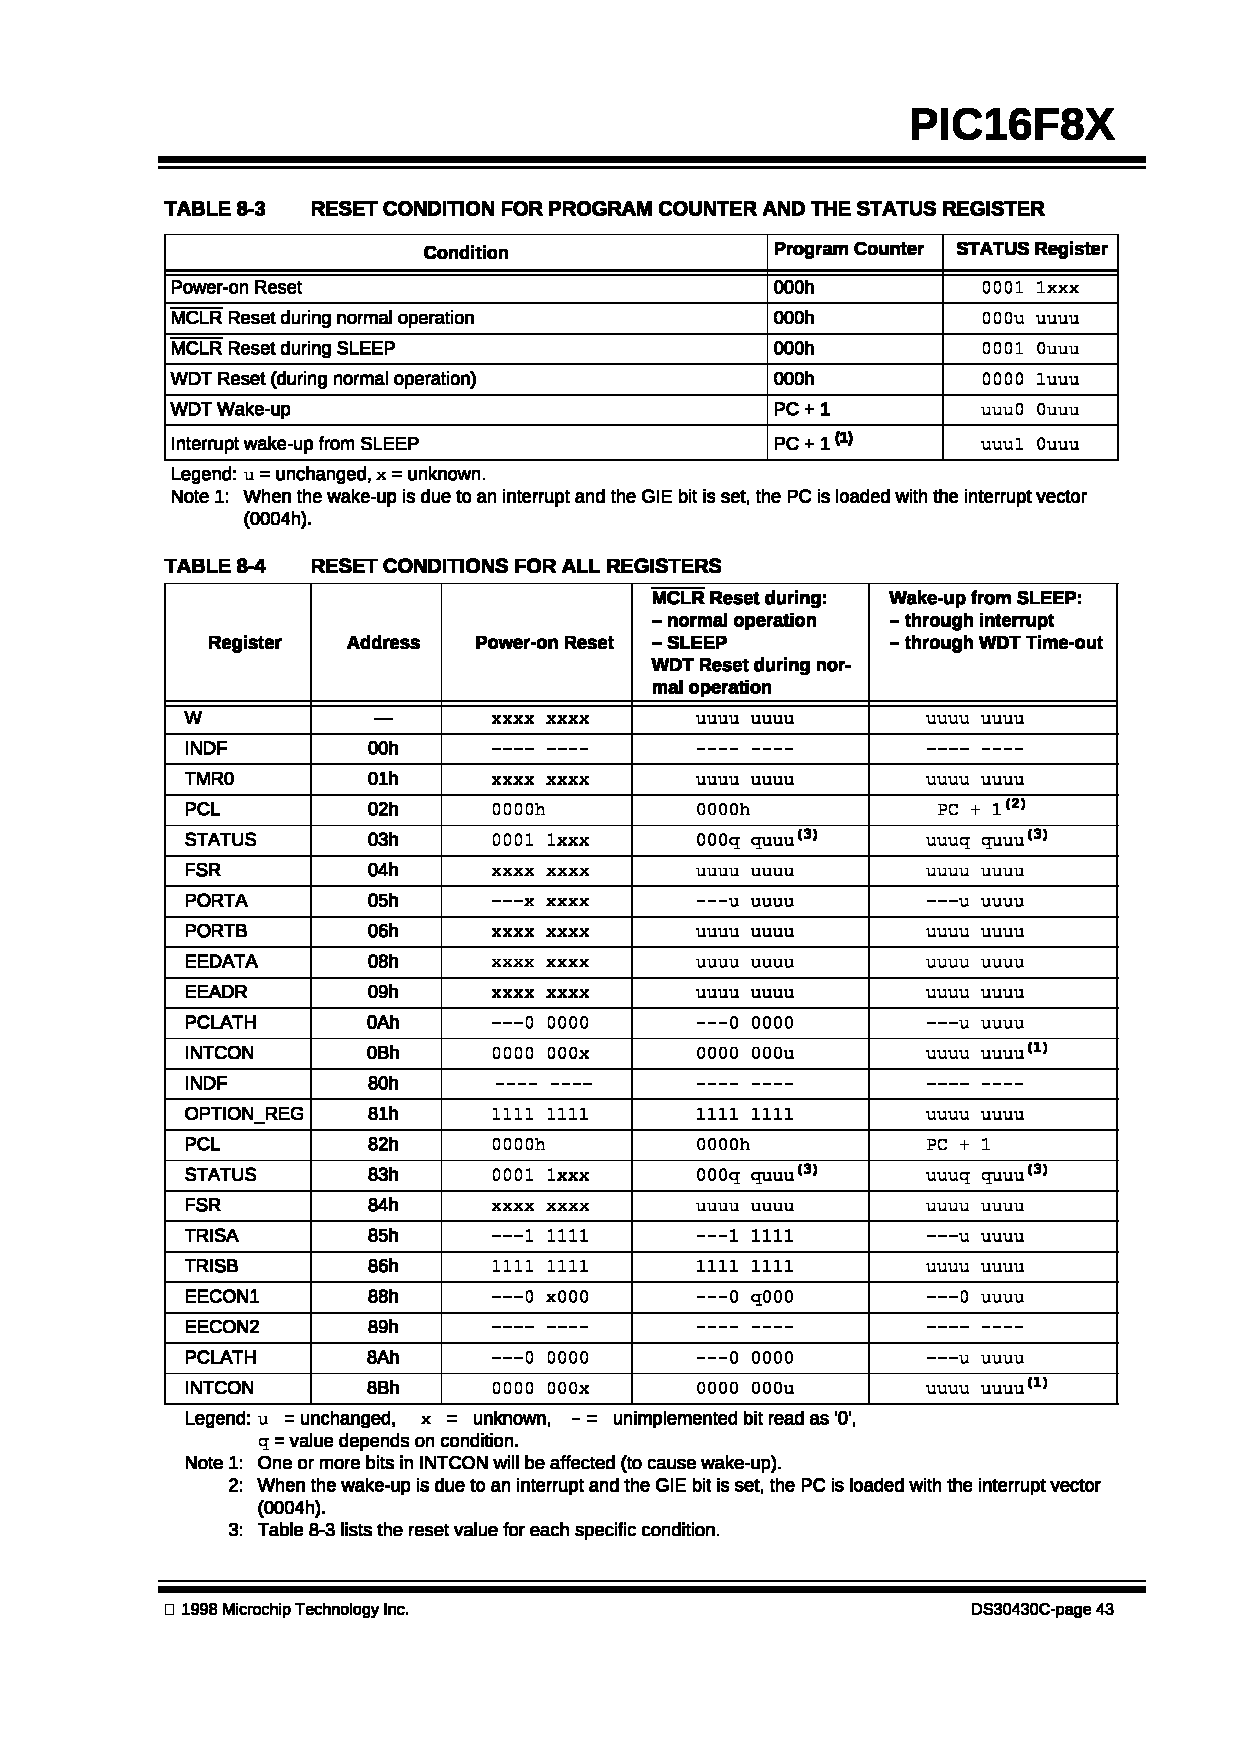
\includepdf[pages={1}]{inputs/Registerverzeichnis.pdf}
  \subsubsection*{PORT RA und TRIS RA Initialisierungssequenz}
  \begin{lstlisting}[language={[x86masm]Assembler}]
    BSF     status, rp0    ;auf Bank 1 umschalten, dort sind die 
    BCF     trisa, 0       ;TRIS-Register. RA0 wird Ausgang
    BCF     trisa, 1       ;RA1 wird ebenfalls Ausgang
    BCF     status, rq0    ;zurueck auf Bank 0 schalten 
    ... 
    ... 
    BSF     porta, 0       ;setzt den Pegel an RA0 auf high
    BCF     porta, 1       ;setzt den Pegel an Ra1 auf low

    \end{lstlisting}
\subsubsection*{Vergleich zweier Speicherstellen}
\begin{lstlisting}[language={[ARM]Assembler}]
  MOVF    adr1, W         ;ein Argument ins W-Register holen
  XORWF   adr2, W         ;XOR verknuepfen und Ergebnis in 
                          ;W-Register, so bleiben adr1 und 
                          ;adr2 unveraendert
  BTFSC   status, Zflag
  GOTO    sindGleich
  GOTO    sindUngleich
  \end{lstlisting}
\subsubsection*{Vergleich zweier Speicherstellen auf größer / kleiner}
\begin{lstlisting}[language={[mips]Assembler}]
  MOVF    adr1, W         ;ein Argument ins W-Register holen
  SUBWF   adr2, W         ;subtrahiere W von Inhalt von adr2
                          ;und schreib Ergebnis ins 
                          ;W-Register, so bleiben adr1 und adr2
                          ;unveraendert
  BTFSC   status,Zflag
  GOTO    sindGleich
  BTFSC   status, CFlag
  GOTO    kleiner         ;es gab einen Ueberlauf im Carry
  GOTO    groesser        
  \end{lstlisting}
\subsubsection*{5 Multiplikator}
In \texttt{HWert1} steht wie viele überläufe es gab.51
\begin{lstlisting}[language=avr]
CLRF    HWert1      ;Loescht HWert1
BCF     status, 0   ;Carryflag wird geloescht Carryflag ist auf 0
MOVF    LWert1, w   ;LWert in das W-Register
RLF     LWert1      ;verdoppelt den LWert
RLF     HWert1      ;moeglicher Ueberlauf der Operation wird in 
                    ;HWert von rechts geschoben. Im Carray steht 0.
RLF     LWert1      ;verdoppelt den LWert
RLF     HWert1      ;moeglicher Ueberlauf der Operation wird in 
                    ;HWert von rechts geschoben. Im Carray steht 0.
ADDWF   LWert       ;Der urspruengliche LWert wird noch dazu addiert
BTFSC   status, 0   ;Es wird geprueft ob Carry 0 ist wenn nicht 
INCF    HWert1      ;wird HWert1 inkrementiert.
\end{lstlisting}


\input{inputs/16-Bit-Zähler + Addierer.tex}
\section*{Eingangsimpuls erfassen }
Schreiben Sie ein Assemblerprogramm für den 16C83, das einen Eingangsimpuls (0,1 ms bis 0,5
ms) erfasst und daraus einen 8 x so langen Ausgangsimpuls erzeugt. Der Ausgangsimpuls soll erst
dann erscheinen, wenn der Eingangsimpuls wieder weg ist. Die Quarzfrequenz beträgt 4 MHz; ein
einfacher Befehl benoetigt somit 1 $\mu s$.\\
\texttt{Pegel prüfen bis eine $1$ kommt}
\begin{lstlisting}[language={[mips]Assembler}]
Label1
  BTFSC   porta, 0
  GOTO    Label1      ;warten auf low
Label2
  BTFSS   porta, 0
  GOTO    Label2      ;wenn das ueberspringt gab es eine ssteigende Flanke
                      ;Ab jetzt messen -> solange incrementieren
\end{lstlisting}
\texttt{8-bitzähler geht bis 512 $\mu s$}
\begin{lstlisting}[language={[mips]Assembler}]
Label3
  INCF    Dauer, 1    ;1 Takt
  BTFSC   porta, 0    ;1
  GOTO    Label3      ;2 Vier Takte fuer den letzten 3
   
  \end{lstlisting}
  \texttt{Ausgabe}
\begin{lstlisting}[language={[mips]Assembler}]
Label3
  MOVLW   8           ;ein Register wird auf 8 gesetzt
  MOVWF   Schleife    ;ist eine Variable
  BSF     porta, 1   
Label5
  MOVF    Dauer, W
  MOVWF   Counter
Label4
  DECF    Counter
  BTFSS   status,zero
  GOTO    Label4
  DECTSZ  Schleife
  GOTO    Label5
  BCF     porta, 1
  GOTO    Label2
\end{lstlisting}
\input{inputs/PIC-Programmierung Übungsaufgabe Nr 1.tex}
\input{inputs/Gib das Bild eines Würfels aus.tex}

\subsubsection*{Binärcodierer ohne Interrupt}
\begin{lstlisting}[language=avr]
  ;*******************************************************
  ; Binarycounter.src
  ;*******************************************************
    device 16f84
  ;Symbol definieren
  status    equ 3
  zero      equ 2
  rp0 	    equ 5
  trisa	    equ 5
  trisb	    equ 6
  porta	    equ 5
  portb	    equ 6

  ;Hex-Zahlen: h am Ende, bei Zahlen mit Buchstaben an erster Stelle eine 0 davor
  wert	    equ 0ch
  alterw	  equ 13
  counter   equ 14
  
  
  org       0
    
  ;Einsprung beim Einschalten (Power on)
  cold
    bsf	    status,rp0	;auf Bank 1 umschalten
    movlw	  0
    movwf	  trisb		    ;PortB wird komplett als Ausgang geschaltet
    bcf 	  trisa,3		  ;RA3 wird Ausgang (Carry)
    bcf	    status,rp0	;zurueck auf Bank 0
  
  ;Definieren von alterw mit aktuellem Wert an RA0
    movf	  porta,w		  ;PortA lesen
    andlw	  00000001b
    movwf	  alterw

  ;Hauptschleife
  loop
    clrf	  counter		  ;Reset und Startwert
    clrf	  portb

  loop1
  ;Reset aktiv?
    btfss	  porta,1		  ;Reseteingang
    goto 	  loop
  ;Inhibit aktiv?
    btfsc	  porta,2		  ;Inhibiteingang
    goto 	  loop1
  
  ;Takteingang lesen
    movf	  porta,w		  ;PortA komplett eingelesen
    andlw	  1		        ;Nur R0 ist von Interesse
  
    xorwf	  alterw,w	  ;Wenn beide gleich, keine Flanke
    btfsc	  status,zero	;Beide gleich, Zero gesetzt
    goto	  loop1		    ;Nichts passiert
    movlw   1
    xorwf	  alterw		  ;Beinhaltet neuen Pegel an RA0
    btfss	  alterw,0
    goto	  loop1
  
  ;Richtige Flanke gefunden
  zuruecksetzen
    incf    counter       ;Zaehler erhoehen
    movlw   0fh
    andwf   counter,w
    xorlw   10            ;Vergleich untere 4 Bits mit 10
    btfss   status,zero
    goto    ausgabe
    movlw   6
    addwf   counter
    movlw   0a0h
    xorwf   counter,w
    btfss   status,zero
    goto    ausgabe
    clrf    counter
    bsf     porta,3
 ;ausgabe auf 7-Segmentanzeige 
  ausgabe
    movf    counter,w     ;zuerst rechte Stelle anzeigen
    call    convert       ;in 7-Segmentanzeige umsetzen
    movwf   portb
    bcf     porta,4       ;Digit einschalten
    bsf     porta,4       ;Digit wieder 
  ausschalten
    swapf   counter,w     ;jetzt linke Stelle anzeigen
    call    convert
    movwf   portb
    bcf     porta,5
    bsf     porta,5
    goto    loop1
  
 ;setzt Binaerzahl in Bitmuster fuer 7-Segmentanzeige um.
  convert
    andlw   15
    addwf   pcl           ;w= offset der zum PCL addiert wird.
    retlw   3fh           ;0
    retlw   06h           ;1
    retlw   5bh           ;2
    retlw   4fh           ;3
    retlw   66h           ;4
    retlw   6dh           ;5
    retlw   7dh           ;6
    retlw   07h           ;7
    retlw   7fh           ;8
    retlw   6fh           ;9
    retlw   0             ;ungueltig
    retlw   0
    retlw   0
    retlw   0
    retlw   0
    retlw   0
  
  end

\end{lstlisting}
\subsubsection*{Interrupts}
\lstinputlisting{inputs/Programme/Interrupt.src}
\subsection*{Binarycounter with Interrupts}
\lstinputlisting{inputs/Programme/Binarycounter with Interrupt.src}
\subsubsection*{AUFGABE 12 Delay}
\lstinputlisting{inputs/Programme/Testprog7.src}
%\subsubsection*{Setzten von Ports}
Wahrscheinlisch Falsch kann morgen noch überarbeitet werden
\begin{lstlisting}[language=avr]
    device 16f84

    trisa			equ		5	;fileadresse
    trisb			equ		6 
    porta			equ		5
    portb			equ		6
    status 		equ 		3
    rp0			equ 		5	;bitadresse
    realcounter	      equ 		13
    counter		equ		12
    pcl               equ         7
    
        org  0
    
    cold
    
    Start
        BSF     status, rp0     
        MOVLW   0
        MOVWF   trisb           ;RB0-RB7 wird Ausgang
        BSF     trisa, 0        ;RA0 wird Eingang
        BCF     status, rp0
    
    Hauptprogramm
        ;CLRF   RB              Setz alle Ausgaenge auf 0
        BTFSS   porta, 0           
        GOTO    Hauptprogramm
        CLRF    counter         ;setzt counter auf 0
        INCF    counter         ;bring counter auf 1
        MOVLW   counter
        MOVWF   realcounter    ;setzt real_counter auf counter
        CLRW                    ;setzt W-Register auf 0
        GOTO    Schleife
    
    Schleife
        BTFSS   porta, 0           ;Wenn Schaltet zu ist wird geskipt
        GOTO    Hauptprogramm
        BTFSC   counter, 0      ;Wenn das Bit 
        GOTO    Ausgabe
        ADDLW   1
        RRF     counter
        GOTO    Schleife
    
    Ausgabe
        CALL    Tabelle
        MOVWF   portb
        INCF    realcounter
        MOVLW   realcounter
        MOVWF   counter
        CLRW
        GOTO    Schleife
        
    Tabelle
        ;ANDLW   15
        ADDWF   02
        RETLW   0000 0000b
        RETLW   0000 0001b
        RETLW   0000 0011b
        RETLW   0000 0111b
        RETLW   0000 1111b
        CLRF    realcounter
        RETLW   0001 1111b	
        RETLW   0
        RETLW   0
        RETLW   0
        RETLW   0
        RETLW   0
        RETLW   0
    
    end

\end{lstlisting}

%\subsubsection*{Testprog2}
%\lstinputlisting{inputs/Programme/Testprog2(1).src}
%\subsubsection*{Testprog3}
%\lstinputlisting{inputs/Programme/Testprog3.src}
%\subsubsection*{Testprog4}
%\lstinputlisting{inputs/Programme/Testprog4.src}
%\subsubsection*{Testprog5}
%\lstinputlisting{inputs/Programme/Testprog5(1).src}
%\subsubsection*{Testprog6}
%\lstinputlisting{inputs/Programme/Testprog6.src}



    

    






\end{document}
